\documentclass[12pt,english]{scrartcl}

\usepackage{amsmath,amssymb}
%\usepackage[amssymb]{SIunits}
\usepackage{babel}
\usepackage[latin1]{inputenc}
\usepackage{graphicx}
\usepackage{color}
\usepackage{url}

\title{KOGW-PM-KNP: Tutorial 2 - G{\"u}nt{\"u}rk{\"u}n's Magpies}
% \author{}
% \date{\today}

\begin{document}

% \maketitle

\begin{center}
\textbf{\begin{LARGE}KOGW-PM-KNP:\\ \vspace{3mm} Tutorial 5 - Quiroga's grandmother aka Jennifer Aniston neuron                                                    \end{LARGE}}
\end{center}

In this tutorial we want to address the question how objects are represented in the brain. The region of cortex bordering the primary visual cortex (= V1, striate cortex) is called extrastriate cortex. It contains multiple areas that are involved in visual processing. After extrastriate cortex, processing of object information is split into two pathways: vision for action and vision for identification, or ``where" and ''what". The``what" pathway continues along inferotemporal (IT) cortex in monkeys or medial temporal lobe (MTL) in humans and involves cortical areas such as the entorhinal cortex or hippocampus that are associated with memory function. The structure of the receptive fields of neurons becomes increasingly complex as one moves from striate to IT cortex. This suggests a hierarchical model of visual perception in which the small receptive fields and simple features of visual cortex are combined with ever-greater complexity culminating in a cell that might fire when you see your own grandmother. The term \textit{grandmother cell} is jargon of the field and refers to any cell that is selectively responsive to one specific object.
The paper by Quiroga, Reddy, Kreiman, Koch \& Fried (2005) reports evidence for exactly such cells. Please read the paper and answer the following questions which should help you to evaluate the implications of their finding. Please work in pairs. 

\begin{figure}[htbp]
\begin{center}
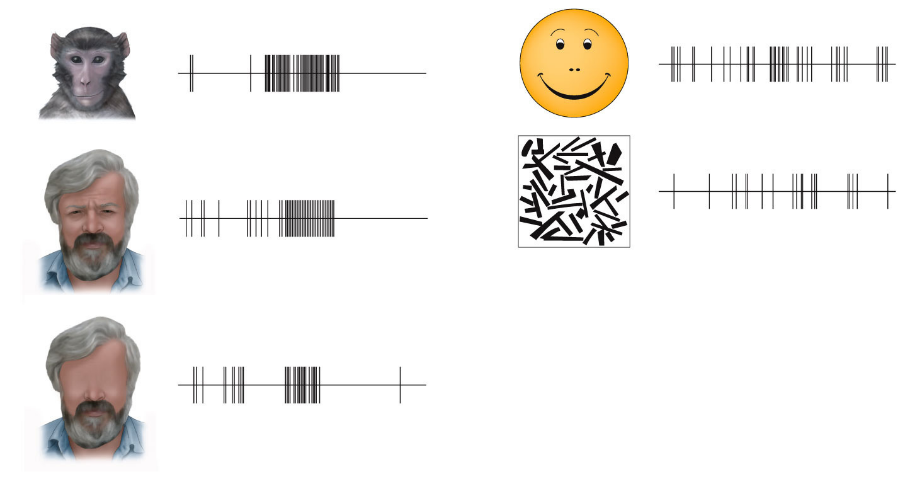
\includegraphics[width = 0.8\textwidth]{IT_cell.png}
\end{center}
\caption{
\label{fig:IT_cell}}
\end{figure}

\begin{enumerate}
 \item What do the authors mean by \textit{invariance}. Explain the concept using Figure \ref{fig:IT_cell} as an example. 
 \item Describe the testing procedure used in the study.
 \item Describe the main result.
 \item What potential confound do the authors identify and how do they rule it out? 
 \item What are the two extreme alternatives for how the brain could represent objects? What are benefits and drawbacks of each alternative? Can you think of a better third alternative? 
\item Is there an alternative explanation for the finding instead of single neurons being the neural substrate that recognizes grandma?
 \item For a critical evaluation of the concept by Terrence Sejnowski read the following \url{https://www.edge.org/response-detail/25325}.
\end{enumerate}

\end{document}
